%%%%%%%%%%%%%%%%%%%%%%%%%%%%%%%%%%%%%%%%%
% University/School Laboratory Report
% LaTeX Template
% Version 3.1 (25/3/14)
%
% This template has been downloaded from:
% http://www.LaTeXTemplates.com
%
% Original author:
% Linux and Unix Users Group at Virginia Tech Wiki 
% (https://vtluug.org/wiki/Example_LaTeX_chem_lab_report)
%
% License:
% CC BY-NC-SA 3.0 (http://creativecommons.org/licenses/by-nc-sa/3.0/)
%
%%%%%%%%%%%%%%%%%%%%%%%%%%%%%%%%%%%%%%%%%

%----------------------------------------------------------------------------------------
%	PACKAGES AND DOCUMENT CONFIGURATIONS
%----------------------------------------------------------------------------------------

\documentclass{article}

\usepackage[version=3]{mhchem} % Package for chemical equation typesetting
\usepackage{siunitx} % Provides the \SI{}{} and \si{} command for typesetting SI units
\usepackage{graphicx} % Required for the inclusion of images
\usepackage{natbib} % Required to change bibliography style to APA
\usepackage{amsmath} % Required for some math elements 
\usepackage{caption}
\usepackage{subcaption}
\usepackage{listings}
\usepackage{color}
 
\definecolor{codegreen}{rgb}{0,0.6,0}
\definecolor{codegray}{rgb}{0.5,0.5,0.5}
\definecolor{codepurple}{rgb}{0.58,0,0.82}
\definecolor{backcolour}{rgb}{0.95,0.95,0.92}
 
\lstdefinestyle{mystyle}{
    backgroundcolor=\color{backcolour},   
    commentstyle=\color{codegreen},
    keywordstyle=\color{codepurple},
    numberstyle=\tiny\color{codegray},
    stringstyle=\color{codepurple},
    basicstyle=\footnotesize,
    breakatwhitespace=false,         
    breaklines=true,                 
    captionpos=b,                    
    keepspaces=true,                 
    numbers=left,                    
    numbersep=5pt,                  
    showspaces=false,                
    showstringspaces=false,
    showtabs=false,                  
    tabsize=2
}
\lstset{style=mystyle}

\setlength\parindent{0pt} % Removes all indentation from paragraphs

\renewcommand{\labelenumi}{\alph{enumi}.} % Make numbering in the enumerate environment by letter rather than number (e.g. section 6)

\newcommand\tab[1][0.5cm]{\hspace*{#1}}

%\usepackage{times} % Uncomment to use the Times New Roman font

%----------------------------------------------------------------------------------------
%	DOCUMENT INFORMATION
%----------------------------------------------------------------------------------------

\title{COMP 429/529: Project 2} % Title

\author{Berkay \textsc{Barlas}} % Author name

\date{\today} % Date for the report

\begin{document}

\maketitle % Insert the title, author and date

\begin{center}
\begin{tabular}{l r}
Date Performed: & March 17, 2019 \\ % Date the experiment was performed
Instructor: & Didem Unat % Instructor/supervisor
\end{tabular}
\end{center}

% If you wish to include an abstract, uncomment the lines below
% \begin{abstract}
% Abstract text
% \end{abstract}

%----------------------------------------------------------------------------------------
%	SECTION 1
%----------------------------------------------------------------------------------------

\tab In this assignment I implemented MPI and OpenMP versions
on top of given serial version for Cardiac Electrophysiology Simulation and conducted experiments. 
\newline
\newline
In this assignment I have completed
\begin{itemize}
    \item 1D MPI version of Cardiac Electrophysiology Simulation
    \item 2D MPI version of Cardiac Electrophysiology Simulation
    \item 2D MPI+OpenMP version of Cardiac Electrophysiology Simulation
    \item Performance Studies for Part a, b, c, d, e
\end{itemize}

\section{Implementation}
\tab In the first part of this assignment I implemented 
a parallel version of a simple image blurring algorithm with
OpenMP which takes an input image and outputs a blurred image.
\\
\tab I used \#pragma omp for collapse() in getGaussian(), loadImage(), saveImage(), applyFilter(), averageRGB() 
methods since all of have nested for loops that can be parallelized. The biggest nested for loop is in applyFilter() 
and it can be parallelizable as below. collapse(5) can not be used because last two for loops depends on previous loops.
\begin{lstlisting}[language=C]
    s
\end{lstlisting}

%----------------------------------------------------------------------------------------
%	SECTION Studies
%----------------------------------------------------------------------------------------
\newpage

\section{Studies}
\subsection{Part A: Strong Scaling}
\begin{description}
    \item[optimal processor geometry: ] \hfill \\ 
    
\end{description}

\textbf{Results}

\begin{figure}[!htb]
    \centering
    \begin{subfigure}{.45\textwidth}
        \centering
        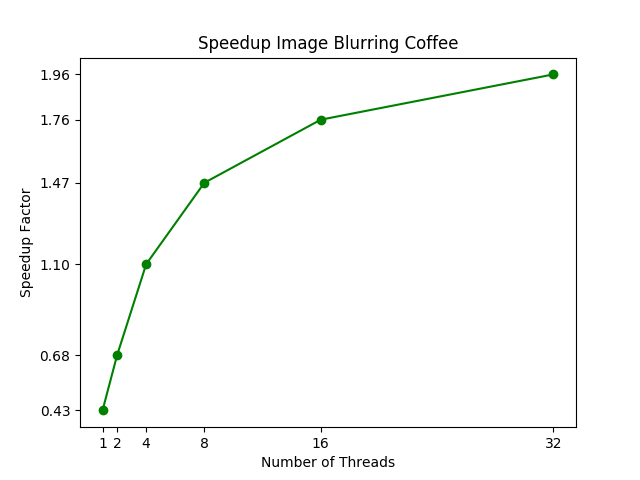
\includegraphics[width=1\linewidth]{./img/speedup_part_1_A.png}
        \caption{Speedup results for the blurring on coffee image.}
    \end{subfigure} 
    \begin{subfigure}{.45\textwidth}
        \centering
        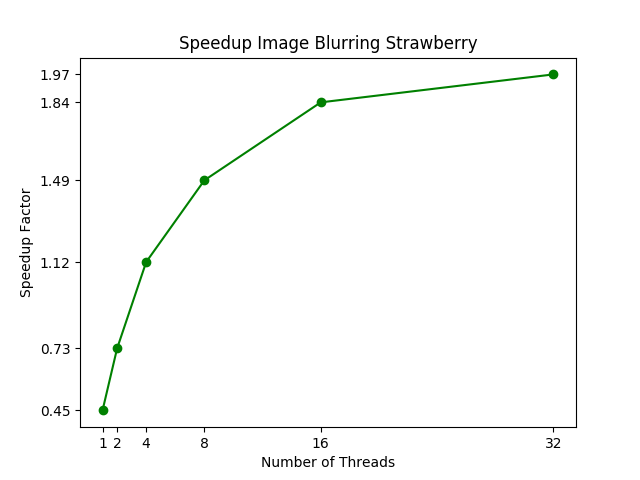
\includegraphics[width=1\linewidth]{./img/speedup_part_1_A_strawberry.png}
        \caption{Speedup results for the blurring on strawberry image.}
    \end{subfigure}
    \caption{Speedup figures for image blurring application}
\end{figure}   

\textbf{Explanation}
\\

\newpage


\subsection{PART B: Strong Scaling with ntasks-per-node=16}
\tab In the second part of this assignment, 
\begin{lstlisting}[language=C]
if(matrix[row][col] != EMPTY) {

}		
\end{lstlisting}
\newpage

\subsection{Part C: Disabling Communication}
\begin{description}
    \item[optimal processor geometry: ] \hfill \\ 
    
\end{description}

\subsection{Part D: Single and Dual node Performance with OpenMP}
\begin{description}
    \item[optimal processor geometry: ] \hfill \\ 
    
\end{description}

\subsection{Part E: Disabling Communication}
\begin{description}
    \item[optimal processor geometry: ] \hfill \\ 
    
\end{description}

\subsection{Tests on Sudoku Problems of Different Grids}
\begin{description}
\item[Part-B]
\end{description} 

\begin{figure}[!htb]
    \centering
    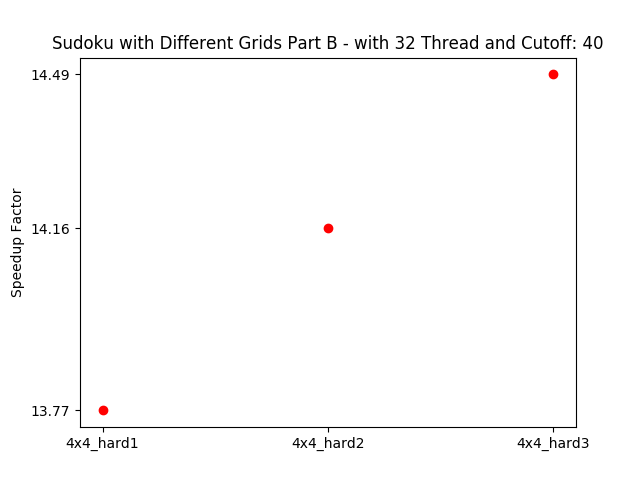
\includegraphics[width=1\linewidth]{./img/grids_part_2_B.png}
    \caption{Results for the 32 Thread Parallel Sudoku solver in Part B with different sizes and difficulties.}
\end{figure}
\tab When the difficulties of sudoku problem increases parallized algorithm in Part B performs better 
over serial serial version. Effectiveness of parallization increases beacuse when the task difficulty
increased the execution time ratio of parallelizable partion over non-parallelizable partion increases. 

%----------------------------------------------------------------------------------------
%	SECTION 6
%----------------------------------------------------------------------------------------

\section{Formulas Used}

\begin{enumerate}
\begin{item}
    \emph{Speedup} 
    \begin{equation*}
    Speedup  = \frac{\mathrm{T1}}{\mathrm{Tp}}
    %\begin{center}\ce{}\end{center}
    \end{equation*}
\end{item}
\begin{item}
    \emph{Amdahl's Law} 
    \begin{equation*}
    Tp \geq Wserial + \frac{\mathrm{Wparallel}}{\mathrm{P}}
    %\begin{center}\ce{}\end{center}
    \end{equation*}
\end{item}
\end{enumerate}




\end{document}